\section{Problema 1: Puentes sobre lava caliente}

\subsection{Presentaci\'on del problema}
%aca ponemos una interpretacion de lo que nos pide el enunciado y algunas aclaraciones de como vamos a encarar el problema.
Se quiere atravesar un puente con $n$ tablones dando saltos acotados por un valor de $x$ tablones. Se empieza afuera del puente y se pretende salir completamente de éste, es decir que como mínimo hay que saltar una vez (en el caso trivial de que $x > n$). La dificultad consiste en que ciertos tablones conocidos están rotos, y no pueden ser pisados. Lo que pide el problema es minimizar la cantidad de saltos para atravesar el puente, o aclarar que es imposible. Los puentes estarán definidos como $t_1$ $t_2$ $...$ $t_n$ donde $t_i = 0$ si el tablón está sano o $t_i = 1$ si está dañado. \\
Por ejemplo, podríamos tener el puente 0 1 0 0 con un salto máximo igual a 2. Como se arranca afuera, saltar al primer tablón se considera como un salto de 1 tablón. En este caso no podemos saltar los dos tablones permitidos porque el segundo tablón está roto (el puente, usando $X$ para marcar donde estamos parados, se vería así: X 1 0 0). El segundo salto sí podremos saltar los 2 tablones, quedando 0 1 X 0, y con el tercer salto saldremos del puente. \\
Una configuración más complicada podría ser el puente 0 0 1 0 0 0 1 1 0 0 para un salto máximo de 3 tablones, ya que ahora tenemos dos posibilidades: saltar al primer o al segundo tablón. Usaremos un algoritmo goloso para resolver el problema (saltar la mayor cantidad posible de tablones) y demostraremos que es correcto y que es la solución óptima para el problema.


\subsection{Resoluci\'on}
\subsubsection{Algoritmo}
%aca ponemos una descripcion de nuestro algorimtmo, presentamos la variables las estructuras y decimos que hacemos.
Dado este problema de optimización planteamos resolverlo con un algoritmo goloso, que consiste en seguir ''una heurística consistente para elegir la opción óptima en cada paso local con la esperanza de llegar a una solución general óptima'' [Cormen p.414 (Greedy Algorithms)].
El problema a optimizar es encontrar la mínima cantidad de saltos para cruzar el puente, y la decisi\'on golosa o la opcion \'optima en cada paso local es elegir el tablon m\'as lejano que pueda alcanzar el participante de acuerdo al rango de salto que tenga. 

El algoritmo recibe un vector con los tablones del puente (puente$[i]$) y un entero que representa el máximo salto que puede dar el participante (\textit{maxSalto}).

Teniendo esa informaci\'on inicializamos la variable \textit{actual} y \textit{proximo} en $0$, que son enteros. La primera representa en que posici\'on del puente se ubica el participante y la segunda la posici\'on del salto m\'as lejano que puede alcanzar a un tablon.
Estas variables son actualizadas por un ciclo, que en el caso que haya soluci\'on corre hasta que la posici\'on \textit{actual} sea mayor a la cantidad de tablones, es decir que el participante haya cruzado el puente.

Dentro del ciclo, se calcula la variable \textit{proximo} con una funci\'on (\textit{calcularProximoTablon}) que recibe el \textit{puente} la posici\'on \textit{actual} y el \textit{maxSalto} y prueba desde el salto m\'as largo que puede dar hasta el m\'inimo cual es el pr\'oximo tablon \'optimo, si no existe, entonces devuelve una excepci\'on y hace que el algoritmo termine o en caso contrario el ciclo lo guarda en un vector de \textit{saltos}.
\textit{Actual} se actualiza a la posici\'on \textit{proximo} en cada iteraci\'on que significa que el participante avanza en cada vuelta del ciclo.

Una vez que termina el ciclo el algoritmo devuelve el arreglo de \textit{saltos}, que es vacio si no existe soluci\'on.

\subsubsection{Pseudoc\'odigo}
%aca va el pseudocodigo del problema.
\begin{algorithm}[H]
\begin{algorithmic}[1]
%\STATE input: vector$<$int$>$ puente, int maxSalto 
%\STATE output: vector$<$int$>$ saltos
\STATE int cantidadTablones $\gets |puente| - 2$ \textcolor{CadetBlue}{// El vector tiene dos tablones más: tanto el primero como el último se consideran fuera del puente}
\STATE int actual $\gets 0$
\STATE int proximo $\gets 0$
\WHILE {actual $\leq$ cantidadTablones}
    \STATE proximo $\gets$ calcularProximoTablon(puente, actual, maxSalto)
    \IF {proximo $==$ $-1$}
        \RETURN vector vacío
    \ENDIF
    \STATE introducirAlFinal(saltos, proximo)
    \IF {proximo $>$ cantidadTablones}
        \RETURN saltos
    \ENDIF
    \STATE actual $\gets$ proximo
\ENDWHILE
\caption{cruzarPuente(vector$<$int$>$ puente, int maxSalto ) $\rightarrow$ vector$<$int$>$ saltos}
\end{algorithmic}
\end{algorithm}

\begin{algorithm}[H]
\begin{algorithmic}[1]
\STATE int cantidadTablones $\gets |puente| - 2$
\WHILE {maxSalto $>$ 0}
    \IF {actual $+$ maxSalto $>$ cantidadDeTablones}
        \RETURN cantidadDeTablones $+$ 1
    \ENDIF
    \IF {puente$[$actual $+$ maxSalto$]$ $==$ 0}
        \RETURN actual $+$ maxSalto
    \ENDIF
    \STATE maxSalto $\gets$ maxSalto $-$ 1
\ENDWHILE
\RETURN $-1$
\caption{int calcularProximoTablon(vector$<$int$>$ puente, int actual, int maxSalto )}% $\rightarrow$ int proximo}
\end{algorithmic}
\end{algorithm}
\subsection{Demostraci\'on}
%aca va la demostracion formal del problema refiriendonos al pseudocodigo o redefiniendo variables (definir todas las cosas de las que vamos a hablar).
%MAXI

Vamos a tratar de probar que dado una secuencia de saltos, si para cada salto $s$, $s$ es un salto m\'aximo, y si la sumatoria de saltos es mayor a la cantidad de tablones del puente, entonces nuestra secuencia es solucion del problema.

Dada un Sec$<$Salto$>$ $se$.

$(\forall i:Nat, i < se.long)(esMax(s,i) \wedge \sum_{j=0}^{se.long-1}se_{j} = puente.long)\implies$ \\ $\not\exists (se':Sec<Salto>) /
se.long < se'.long \wedge \sum_{j=0}^{se'.long-1}se'_{j} \geq puente.long)$  

Donde esMax devuelve true cuando el no existe un salto mas largo desde la posicion donde estamos.
%implementar esto.

Para probar esto, vamos a utilizar la definici\'on can\'onica de demostraci\'on de correctitud para algoritmos greedy, dada en clase por la c\'atedra. Un algoritmo goloso, puede plantearse como el siguiente esquema:
%comentar introduction to algorithim

\begin{algorithm}
\begin{algorithmic}
%\STATE input: S, F, P 
%\STATE output: S
\STATE $S^{opt}$ $=$ $\emptyset$
\WHILE {S $!=$ $\emptyset$}	
    \STATE X = $f(S)$
    \STATE S = $S - {X}$
    \IF {p($S^{opt}$,X)}
    \STATE $S^{opt} = S^{opt} \cup$ ${X}$   
    \ENDIF         
\ENDWHILE
\RETURN $S^{opt}$
\end{algorithmic}
\end{algorithm}

Luego para garantizar la correctitud del mismo hay que garantizar 4 puntos:

%comentar que esta sacada de la clase practica del dia xxxxxxx.
%esto deberia estar con indices, no con numeros cabeza

1) Definimos una noci\'on de lo que significa ser “sub-soluci\'on” de una soluci\'on.

2) Probar que $S^{opt}$ empieza siendo sub-soluci\'on de alguna soluci\'on \'optima.

3) Probar que si  $S^{opt}$ es sub-soluci\'on de alguna soluci\'on \'optima al iniciar 	una iteraci\'on del ciclo, entonces al terminar  esa iteraci\'on, $S^{opt}$ sigue siendo una subsoluci\'on de alguna soluci\'on \'optima.

4) Probar que cuando S $== \emptyset$, $S^{opt}$ es una soluci\'on \'optima.

Bueno para probar estos 4 puntos, primero vamos a definir F, S y P.


S es un conjunto de los saltos que uno puede dar representados por los pares (x,y) de tal que el representa un salto desde la posicion x hasta la posicion y con 0$<$ y-x$\leq$salto m\'ax.
F es una funci\'on selecciona de S el par con mayor diferencia (y - x) y menor coordenada x.
P($S^{opt}$,X) devuelve TRUE cuando el tabl\'on donde cae X no esta roto y cuando el salto no se superpone con un salto anterior.
%Puente[$\sum_{i=0}^{S^{opt}.long}S^{opt}_{j}$ + X] $==$ 0 
%Donde Puente es el array de tablones, donde un tabl\'on esta sano si su valor es 0.
Vamos a definir ser sub-soluci\'on como ser el prefijo de una soluci\'on cuando ordenamos por orden de saltos.
Como la cantidad de saltos que puede darse en un puente es finita, va existir al menos un m\'aximo local y vamos a poder asignarle un cardinal. Entonces como existe al menos un conjunto de saltos de cardinal \'optimo, el conjunto $\emptyset$ empieza siendo sub-soluci\'on de ese conjunto.
Con esto queda comprobado 1) y 2).

Dado $S^{opt}$ sub-soluci\'on al principio del ciclo, queremos garantizar que $S^{opt}$ es sub-soluci\'on al finalizarlo.
Supongamos que $S^{opt}$ es sub-soluci\'on de $S^{*}$ al principio del ciclo.
Bueno si a $S^{opt}$ no le agrego nada, sigue siendo una subsolucio\'on.
Si el caso es en el que agrego X, quiero ver que eso sigue siendo alguna sub-soluci\'on para alg\'un $S'^{*}$. En particular queremos ver que $S'^{*}$ $\subset$ $S^{*}$. 
Si agregamos X, es el caso en donde P dio true, por lo tanto X cae en un tabl\'on que no esta roto y el salto no se superpone con uno anterior.
Adem\'as X era el m\'aximo de los saltos posibles y de menor coordenada x obtenido por F.
Bueno, si X $\in$ $S^{*}$, entonces podemos tomar $S'^{*}$ = $S^{*}$, asi que veamos el caso en que X $\notin$ $S^{*}$.

Ahora tomemos $S'^{*}$ = $S^{*}$ $\cup$ ${X}$
Este conjunto puede tener elementos que se superponen, si no los tiene entonces 
$S'^{*}$ es sub-soluci\'on.
Si los tiene, y ordenamos por orden de salto (primera coordenada) , $S'^{*}$ no puede superponerse con $S^{opt}$ ya que $S^{opt}$ era sub-soluci\'on de $S^{*}$.
Por lo tanto si existe un elemento que se superponga, se superponen con X.
Sea Y un elemento que se superpone con X.
Sean $Y_{1},Y_{2},X_{1},X_{2}$ las componentes de Y,X respectivamente.
$Y_{1}\geq X_{1}$ ya que sino X no tenia la primera componente m\'inima.

Si $Y_{1} = X_{1}$ entonces $X_{2} \geq Y_{2}$ ya que sino F hubiera agarrado primero a Y. Por lo tanto yo podria tomar $S'^{*}$ = $S^{*}$ $\cup$ ${X}$ - ${Y}$ y eso seguiria siendo sub-soluci\'on ya que el intervalo I = [$Y_{2},X_{2}$] estar\'ia cubierto con un solo salto por un soluci\'on que contenga a X, y necesitaria al menos 2 para un soluci\'on que contega a Y.

Si $Y_{1} > X_{1}$ entonces hay dos casos:

Si $Y_{2} \leq X_{2}$ entonces todo el intervalo cubierto por Y, estaria inclu\'ido en el intervalo cubierto por X, y en el intervalo I = [$X_{1},Y_{1}$], I $\neq \emptyset$ habr\'ia que cubrirlo con un salto por lo tanto $S^{*}$ no ser\'ia subsoluci\'on. Mismo para I' =  [$Y_{2},X_{2}$].

Si $Y_{2} > X_{2}$ entonces yo se que X,Y no pueden estar en la misma soluci\'on(se superponen). Pero se que Y pertenece a alguna soluci\'on. Veamos que existe un intervalo que cubre X, pero no Y que seria el intervalo I = [$X_{1}$,$Y_{2}$].
Bueno pero como X contiene a todo este intervalo, existe una solucion que contiene al salto $S_{Y}$ = ($X_{1}$,$Y_{2}$). Asi que dado un soluci\'on que contiene a Y, al menos contiene un salto m\'as en ese intervalo. Recordemos que puede haber saltos que extiendan el ultimo salto de $S^{opt}$, pero no nos interesan porque no ser\'ian compatibles con $S^{opt}$ ya que se superpondr\'ian.
 
Luego dado el intervalo I'=[$X_{2}$,$Y_{2}$], como X se superpone con Y, $X_{2}$ $>$ $Y_{1}$, por lo tanto existe y es posible un salto $S_{X}$ con componentes ($X_{2}$,$Y_{2}$).
Luego si analizamos las dos sub-soluciones contienen al mismo intervalo en dos saltos, por lo que si existe una soluci\'on para que contiene a Y, existe una soluci\'on que contenga a X. 

Con esto queda comprobado 3).

Finalmente, si S $== \emptyset$ entonces no hay mas saltos, por lo tanto nuestra $S^{opt}$ recorre todo incluye a todo el puente.
Tenemos $S^{opt}$  que sabemos es una sub-soluci\'on de $S^{*}$. Y si $S^{opt}$ ya recorrio todo el puente, no hace falta agregarle ning\'un salto, por lo tanto $S^{opt} =S^{*}$.  

Con esto queda comprobado 4).
%MAXI
\\
\subsection{An\'alisis de complejidad}
%aca decimos cuanto cuesta cada parte del algoritmo y damos un valor final de la complejidad del algoritmo, ej O(logn).
El algoritmo \textit{cruzarPuentes} se puede dividir en dos partes:
\begin{itemize}
\item Inicialización
\item Ciclo
\end{itemize}

En la Inicialización el algoritmo asigna 3 variables en $O(1)$, con lo cual su complejidad es $3*O(1) = O(1)$
El ciclo, como peor caso, itera hasta $n$ veces, donde $n$ es la \textit{cantidadDeTablones}. Adentro del ciclo se calcula la función \textit{calcularProximoTablon} para cada iteración. Esta nos dice el índice del próximo tablón óptimo para saltar, y a su vez es otro ciclo que se repite $k$ veces haciendo una cantidad acotada de operaciones $O(1)$, donde $k$ es la variable de entrada \textit{maxsalto} que es un valor acotado.
Luego el ciclo continua haciendo asignaciones y condicionales y devoluciones en $O(1)$.

Haciendo el calculo de complejidad obtenemos:

$O($\textit{cruzarPuentes}$) = 3*O(1) + n(O(k))$

Que es lo mismo que:

$O($\textit{cruzarPuentes}$) = O(n*k)$

%esto de decir que el algoritmo depende de k, yo no lo pondria porque sino nos van a decir que no es O(n) como pidieron ellos.

\label{an}
Entonces por cada paso que da, el algoritmo calcula hasta k tablones para saber cual es el pr\'oximo que no este roto m\'aximo, pero con la particularidad que calcula primero el mas lejano, por lo tanto dado un salto de longitud k':Nat, k'$\leq$ k, el pr\'oximo salto S, va a tener que ser mayor o igual a k - k', ya que sino S caeria en un tabl\'on roto.
Esto sucede porque k' esta acotado por los tablones que est\'an rotos.
Por ejemplo, suponiendo un k = 10. Dentro de un intervalo de tablones de 10 elementos, el tabl\'on 10, 9 y 8 est\'an rotos. Por lo tanto k' = 7. Entonces vemos que los tablones rotos por arriba son los que acotan a k', luego el pr\'oximo salto debe ser mayor a 3. Y si se itera mas de k - k' veces, el puente no tiene soluci\'on.
Esto lo que implica que dado cualquier k, el algoritmo siempre va a recorrer a lo sumo N elementos dentro del puente. El peor caso seria k=1.
Finalmente podemos concluir que es de orden $O(n)$.


Podemos ver que el algoritmo depende de $k$, es decir, del \textit{maxsalto} del participante, con lo cual podemos considerar que tiene una complejidad pseudopolinomial ya que depende de una variable de entrada, pero como sabemos que $k$ es acotado por una constante finalmente podemos concluir que es de orden $O(n)$.

\subsection{Test de complejidad}
%aca van los graficos y todos los testeos que hagamos para probar que en la practica el algoritmo cumple la complejidad que propusimos en el punto anterior

Para analizar y testear la complejidad del algoritmo implementado para la resoluci\'on del problema puentes colgantes realizamos los siguientes testeos:

\begin{itemize}
  \item Test de casos de tamaño fijo.
  \item Test de entrada al procesador.
  \item Test de analisis de peor caso.
\end{itemize}

\newpage



\subsubsection{Test de casos de tamaño fijo}


Para el test de complejidad utilizamos un algoritmo que genera un array de boolean aleatorios dado un k:Nat, tal que el largo del array es de tamaño k.

Luego generamos m:Nat arrays aleatorios de tamaño k. Dado un array $a$ se construye un puente $p$ el cual consta de los mismos elementos que el array aleatorio. 

$(\forall i:Nat, i < a.length)(a_{i} == p_{i})$

Luego se llama al algoritmo que obtiene la soluci\'on para ese puente.

Los tiempos medidos son a partir de que se llama al constructor del puente, y hasta despu\'es del llamado a nuestro algoritmo soluci\'on.

Para el test de casos de tamaño fijo, lo que usamos fue dadas las variables 

puenteMax:Nat, saltoMax:Nat, step:Nat, $cantidadDeIteraciones$:Nat. 

Vamos a iterar desde (i$=$step;i$<$puenteMax;i+=step), vamos a hacer $cantidadDeIteraciones$ instancias de puente y luego llamar al algoritmo de resoluci\'on con el procedimiento descrito arriba.

Luego dado un tiempo $T_{i}$ siendo este el promedio de todas las corridas de tamaño i, vamos a realizar un analisis de la complejidad obtenida.

Para el salto s:Nat que va a poder dar cada participante en cada instancia de puente tambien es n\'umero aleatorio tal que

saltoMax:Nat, s $\leq$ saltoMax $\wedge$ saltoMax $<<$ i.

El siguiente gr\'afico muestra el crecimiento del $T_{i}$ en funci\'on de i, es decir el crecimiento del tiempo en funci\'on del crecimiento de elementos.
Los valores utilizados para la generaci\'on del grafico son:

\newpage

$cantidadDeIteraciones$ $=$ 100 step $=$ 50000 puenteMax $=$ 500000000 saltoMax = 10

\begin{figure}[ht]
	\begin{minipage}[t]{\linewidth}
		\centering
		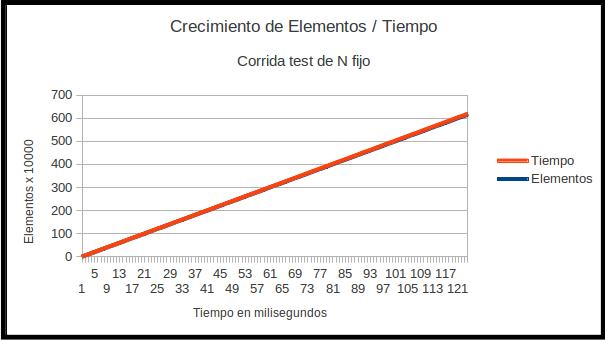
\includegraphics[width=\textwidth]{grafico_de_n_fijo.jpg}
	\end{minipage}	
\end{figure}

Como se puede apreciar la complejidad as\'intotica temporal en este caso, es lineal en el tamaño de la entrada.


\newpage
\subsubsection{Test de entrada al procesador}

El objetivo de este test era correr un test similar al test de tamaño fijo pero evitando los outlayers que pudiera generar el momento de entrada del problema al microprocesador. 

Para ello, lo que se implemento, fue correr una misma instancia de puente k veces y tomar ahora el promedio de esas k corridas similares, realizando el mismo proceso que en el test de tamaño fijo. Luego analizar en un gr\'afico la complejidad temporal de este test.

Los valores utilizados para la generaci\'on de este gr\'afico son:

$cantidadDeIteraciones$ $=$ 10 step $=$ 500000 puenteMax $=$ 500000000 saltoMax = 10 

k $=$ 10


\begin{figure}[ht]
	\begin{minipage}[t]{\linewidth}
		\centering
		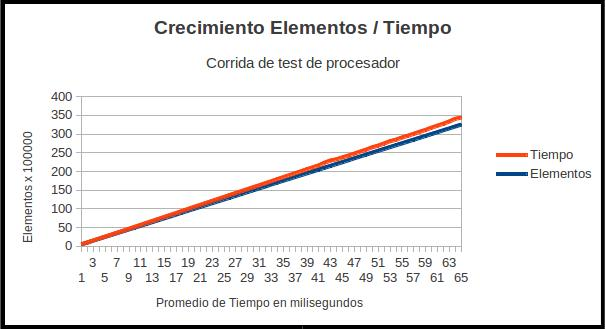
\includegraphics[width=\textwidth]{grafico_de_entrada_al_procesador.jpg}
	\end{minipage}	
\end{figure}

Como se puede apreciar la complejidad as\'intotica temporal en este caso, tambi\'en es lineal en el tamaño de la entrada.


\subsubsection{Test de peor-mejor caso}

Por lo analizado en demostraci\'on de correctitud, el peor caso va a ser cuando el salto m\'aximo s de un participante es s $=$ 1. Ya que este caso, de tener soluci\'on un puente p, se deber\'ia recorrer todos los tablones de p.

Luego la complejidad es exactamente N.

Los mejores casos ser\'ian lo que el salto m\'aximo s de un participante dado un puente p.

s $\geq$ p.largo

Ya que todo puente que el participante pueda saltar de un solo salto, tiene soluci\'on y nuestra implementaci\'on la haya en O(1).

\newpage

 
\subsection{Testing}
%aca ponermos todos nuestros casos bordes, como actua nuestro algoritmo en los casos particulares.

Para analizar y testear la correctitud del algoritmo implementado para la resoluci\'on del problema puentes colgantes realizamos los siguientes testeos:

\begin{itemize}
  \item Test de casos bordes.
  \item Test de archivos est\'aticos.
  \item Test de an\'alisis de input-output.
  \item Test de analisis generador de casos.
\end{itemize}

\subsubsection{Test de casos bordes}

Para los casos bordes de nuestro algoritmo elegimos correr una bater\'ia de test los cuales simulan casos at\'ipicos.
Los siguientes test fueron implementados:
Dado un puente p y participante con salto m\'aximo m.

\begin{itemize}
  \item TestConPuenteConTamanio0() $=$ Chequea soluci\'on para p.largo $=$ 0.
  \item 	TestConSaltoMaximo0() $=$ Chequea soluci\'on para s $=$ 0.
  \item TestConSaltoMaximoMayorAPuente(); Chequea soluci\'on para s $\geq$ p.largo 
  \item testConPuenteNegativo(); $=$ Chequea soluci\'on para p.largo $\leq$ 0
  \item testConSaltoNegativo(); $=$ Chequea soluci\'on para s $\leq$ 0
\end{itemize}

\subsubsection{Test de archivos est\'aticos}

El objetivo de este test era probar la correctitud de nuestra implementaci\'on a partir de un archivo est\'atico de entrada y un archivo est\'atico de salida.
Estos archivos est\'atico de entrada y salida se los puede encontar en el directorio del programa bajo el nombre de "puentes-estatico.txt" para la entrada y "solucion-estatica" para la salida.

%hay que ponerle algunos casos mas a estos archivos%

\subsubsection{Test de an\'alisis de input-output}

El objetivo de este test era probar la correctitud del algoritmo de entrada de datos.
Se buscaba corroborar que la implementaci\'on correspondiera dada un archivo de entrada a la de un puente ya instanciado por el programa.
Para ello se genero un caso de test, el cual dado un puente creado aleatoriamente, crea un archivo de texto similar a los de entrada de la c\'atedra, con este puente. 

Luego se llamo con ese archivo a nuestra implementaci\'on de input, corroborando que la salida de este m\'etodo fuera similar a la de una llamada con el puente ya instanciado.

El test corre con k entradas de puentes generadas aleatoriamente.

\subsubsection{Test generador de casos}

El objetivo de este test es corroborar que dado un puente p, generado aleatoriamente y dada la solucion s. Corroborar que efectivamente si el algoritmo no devuelve soluci\'on entonces efectivamente no existe tal, y si la devuelve entonces s es soluci\'on del problema.

Para probar que no existe una soluci\'on para un puente p, vamos a aprovecharnos de una caracteristica de los puentes sin soluci\'on.

Para todo puente p sin soluci\'on dado un participante con salto m\'aximo m , existe un intervalo de tablones $p_{i}$,$p_{j}$ tal que para todo tabl\'on t dentro de ese intervalo, t est\'a roto.
La comprobaci\'on informal de este enunciado es que si no existies ese intervalo, el participante siempre podria dar saltos al intervalo de tablones rotos que tiene adelante. Por lo tanto podr\'ia saltar por todo el puente.

Entonces dado un puente sin soluci\'on se chequea efectivamente que existe al menos un intervalo.

Para corroborar que una s efectivamente es soluci\'on de p, vamos a iterar por los tablones de s y chequear en p, que estos no esten rotos.
Si bien esto no nos garantiza que s sea optima, nos garantiza que sea soluci\'on.

Una mejora para estos test ser\'ia encontrar una caracter\'istica de s, tal que no asegure que es \'optima. Para ello, podr\'iamos generarnos por fuerza bruta todas las secuencias de saltos posibles y agarrar las que sean soluci\'on y garantizar que nuestra s es mejor o igual que todas las dem\'as.

\subsection{Compilaci\'on y corrida}


La clase la cual debemos correr es Main, y debe tener un par\'ametro de entrada que sea el nombre del archivo del cual vamos a leer. \'Este archivo debe estar en el directorio del proyecto a en la carpeta "TP1-EJ1", a la altura donde estan los dem\'as archivos de texto.
Para correr la clase Main, hay que posicionarse en el directorio bin del proyecto:

cd TP1-P1$/$bin

Luego desde este directorio con el comando java main/Main $<$nombre de archivo$>$.

Ej: TP1-P1$/$bin java main$/$Main ../puente.txt

El output de esto deberia ser: 

3 2 4 6

no

 